\chapter{Abstraction}

\section{LMDPs}

\subsection{Derivation}

\subsubsection{LMDP solutions}

Pick $a \in A$, versus, pick $\Delta(S)$. $f: S\to A$ vs $f:S \to \Delta(S)$.

In the original Todorov paper, they derive the LMDP equations for minimising a cost function. This maximisation derivation just changes a few negative signs around. Although there is also a subtle change in the interpretation of what the unconstrained dynamics are doing. (??? explain)

\begin{align}
V(s) &= \mathop{\text{max}}_{u} q(s) - \text{KL}(u(\cdot| s) \parallel p(\cdot | s)) + \gamma \mathop{\mathbb E}_{s' \sim u(\cdot | s)} V(s') \tag{1}\\
\\
&= q(s) + \mathop{\text{max}}_{u} \bigg[ \mathop{\mathbb E}_{s' \sim u(\cdot | s)} \log(\frac{p(s' | s) }{ u(s' | s)}+\gamma \mathop{\mathbb E}_{s' \sim u(\cdot | s)} \big[V(s')\big] \bigg] \tag{2}\\
\log(z(s)) &= q(s) + \mathop{\text{max}}_{u} \bigg[ \mathop{\mathbb E}_{s' \sim u(\cdot | s)} \log(\frac{p(s' | s) }{ u(s' | s)}+\mathop{\mathbb E}_{s' \sim u(\cdot | s)} \big[\log(z(s')^{\gamma})\big] \bigg] \tag{3}\\
&= q(s) + \mathop{\text{max}}_{u} \bigg[ \mathop{\mathbb E}_{s' \sim u(\cdot | s)} \log(\frac{p(s' | s)z(s')^{\gamma} }{ u(s' | s)} ) \bigg] \tag{4}\\
G(s) &= \sum_{s'} p(s' | s) z(s')^{\gamma} \tag{5}\\
&= q(s) + \mathop{\text{max}}_{u} \bigg[ \mathop{\mathbb E}_{s' \sim u(\cdot | s)} \log(\frac{p(s' | s)z(s')^{\gamma} }{ u(s' | s)} \cdot \frac{G(s)}{G(s)} ) \bigg] \tag{6}\\
&= q(s) + \log G(s) + \mathop{\text{min}}_{u} \bigg[\text{KL}\big(u(\cdot | s) \parallel \frac{p(\cdot | s)\cdot z(\cdot)^{\gamma}}{G(s)} \big) \bigg] \tag{7}\\
u^{* }(\cdot | s) &= \frac{p(\cdot | s)\cdot z(\cdot)^{\gamma}}{\sum_{s'} p(s' | s) z(s')^{\gamma}} \tag{8}\\
\log(z_{u^{* }}(s)) &= q(s) + \log \big(\sum_{s'} p(s' | s) z_{u^{* }}(s')^{\gamma}\big) \tag{9}\\
z_{u^{* }}(s) &= e^{q(s)}\big(\sum_{s'} p(s' | s) z_{u^{* }}(s')^{\gamma}\big) \tag{10}\\
z_{u^{* }} &= e^{q(s)}\cdot P z_{u^{* }}^{\gamma} \tag{11}\\
\end{align}

By definition, an LMDP is the optimisation problem in (1). We can move the $\text{max}$ in (2), as $q(s)$ is not a function of $u$. Also in (2), expand the second term using the definiton of KL divergence, the negative from the KL cancels the second terms negative. (3) Define a new variable, $z(s) = e^{v(s)}$. Also, use the log rule to move the discount rate. (4) Both expectations are under the same distribution, therefore they can be combined. Also, using log rules, combine the log terms. (5) Define a new variable that will be used to normalise $p(s' | s)z(s')^{\gamma}$. (6) Multiply and divide by $G(s)$. This allows us to rewrite the log term as a KL divergence as now we have two distributions, $u(\cdot | s)$ and $\frac{p(\cdot | s)z(\cdot)^{\gamma}}{G(s)}$. (7) The change to a KL term introduces a negative, instead of maximising the negative KL, we minimise the KL. Also in (7) the extra G(s) term can be moved outside of the expectation as it is not dependent in $s'$. (8) Set the optimal policy to minimise the KL distance term. (9) Since we picked the optimal control to be the form in (8), the KL divergence term is zero. (10) Move the log. (11) Rewrite the equations for the tabular setting, giving a $z$ vector, uncontrolled dynamics matrix.

\subsubsection{MDP Linearisation}

The ability to solve LMDPs is great, but it's only useful if we can map MDPs into LMDPs, solve them, and map the solution back.
Our goal here is to find a LMDP that has 'similar' structure to the original MDP we were given. \footnotemark[2]

\footnotetext[2]{This derivation is not the same as in Todorov. He sets $b_a \neq r, b_a = r - \sum P \log P$.}


\begin{align}
\forall s, s' \in S, \forall a \in A, \exists u_a& \;\;\text{such that;} \tag{1}\\
P(s' | s, a) &= u_a(s'|s)p(s'|s) \tag{2}\\
r(s, a) &= q(s) - \text{KL}(P(\cdot | s, a) \parallel u_a(\cdot| s) ) \tag{3}\\
\\
r(s, a) &= q(s) - \text{KL}(P(\cdot | s, a)\parallel\frac{P(\cdot | s, a)}{p(\cdot|s)}) \tag{4}\\
r(s, a) &= q(s) - \sum_{s'}P(s' | s, a) \log(p(s'|s)) \tag{5}\\
\\
m_{s'}[s]&:= \log p(s' | s) \tag{6}\\
D_{as'}[s] &:= p(s'|s, a) \tag{7}\\
c_{s'}[s] &:= q[s] \mathbf 1 - m_{s'}[s] \;\;\text{such that} \;\; \sum_{s'} e^{m_{s'}[s]} = 1 \tag{8}\\
\\
r_a &= D_{as'} ( q \mathbf 1 - m_{s'}) \;\;\forall s \tag{9}\\
r_a &= D_{as'}c_{s'}  \;\;\forall s \tag{10}\\
c_{s'} &= r_aD_{as'}^{\dagger} \;\;\forall s\tag{11}\\
q &= \log \sum_{s'} e^{c_{s'}} \;\;\forall s\tag{12}\\
m_{s'} &= q - c_{s'} \;\;\forall s\tag{14}\\
\end{align}


Therefore we have $|A|$ linear relationships, for each $s\in S$.

(5) KL introduces a negative, but we also use the log rule to move $p(s'|s)$ to the nominator, adding another negative, and thus cancelling. Yielding the cross entropy between .. and ... .

(11) The More-Penrose pseudo inverse. We apply to the RHS... ???.


\subsection{Toy experiments}

\begin{figure}
\centering
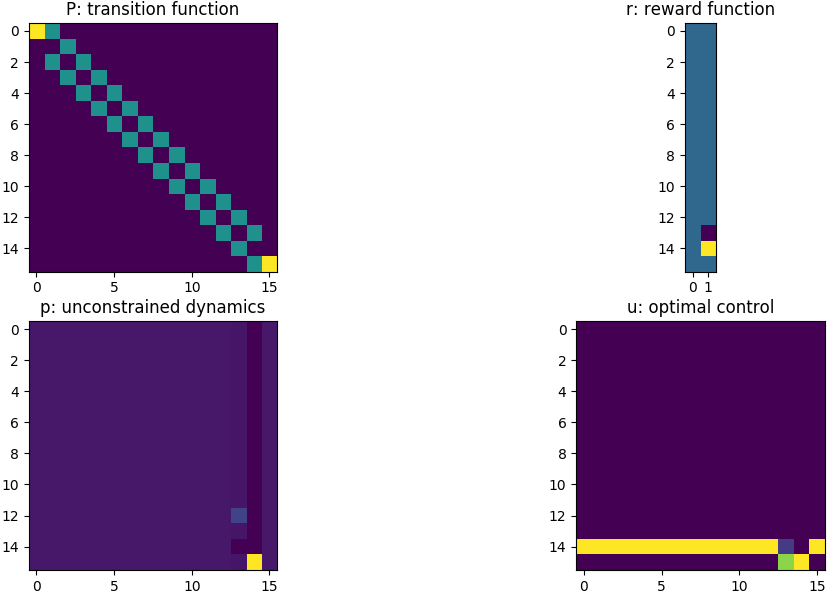
\includegraphics[width=1\textwidth,height=0.35\textheight]{../../pictures/figures/chain-test-zero-rewards.png}
\caption{A chain problem with zero reward on all states except the last two.
The optimal control to this problem is not sensible: in every state, jump to the state with positive reward.
However, it is not possible to make those transitions as }
\end{figure}

\begin{figure}
\centering
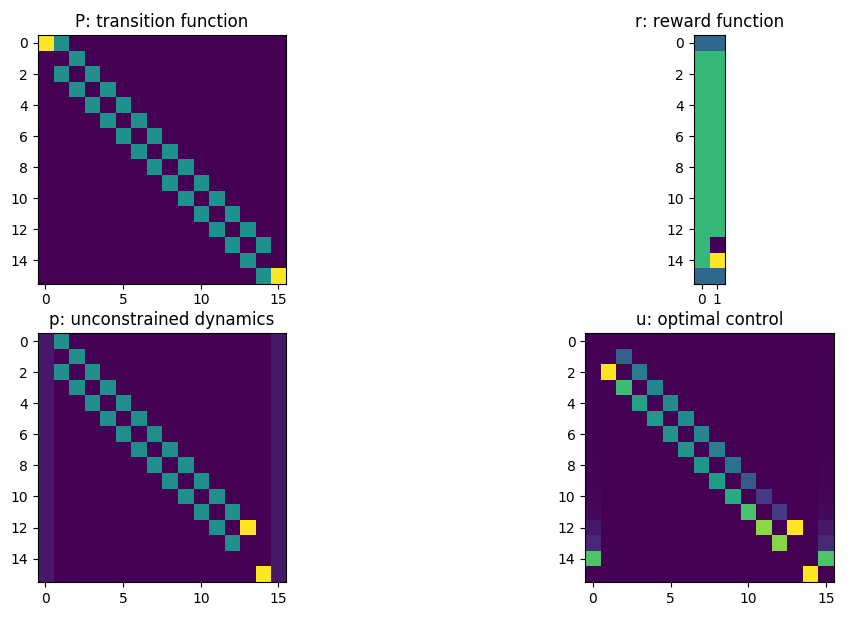
\includegraphics[width=1\textwidth,height=0.35\textheight]{../../pictures/figures/chain-test-pos-rewards.png}
\caption{A chain problem with positive rewards applied to all states.}
\end{figure}

\begin{figure}
\centering
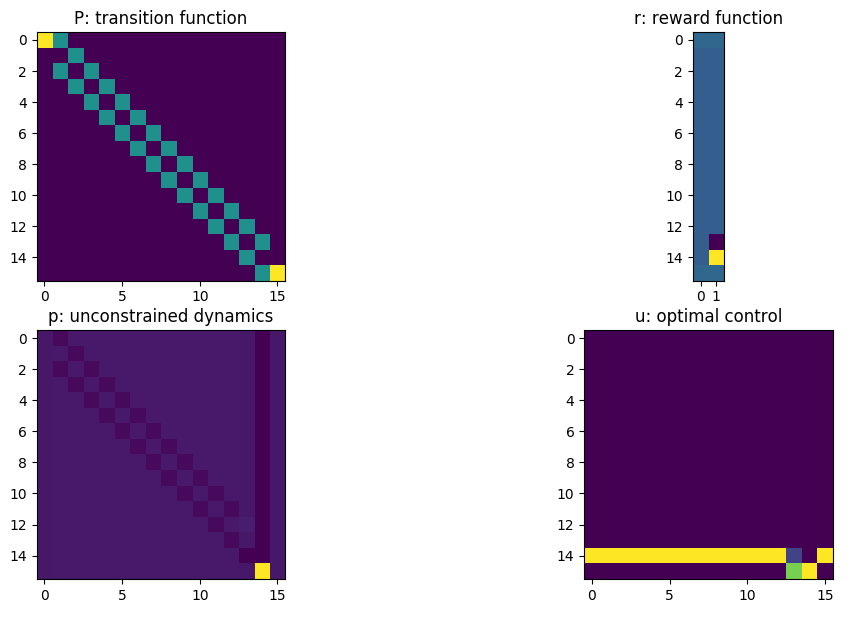
\includegraphics[width=1\textwidth,height=0.35\textheight]{../../pictures/figures/chain-test-neg-rewards.png}
\caption{A chain problem with negative rewards applied to all states}
\end{figure}

The point is, it is not entierly clear how to embed an MDP into a LMDP.


\section{Symmetry}


\hypertarget{mirror-symmetry}{%
\paragraph{Mirror symmetry}\label{mirror-symmetry}}

\begin{figure}
\centering
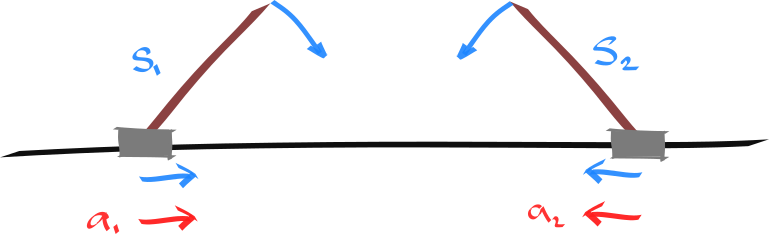
\includegraphics[width=1\textwidth,height=0.25\textheight]{../../pictures/drawings/cart-pole-mirror.png}
\caption{???}
\end{figure}

\begin{align}
\Delta_{\tau}(s, a) = \mathop{\mathbb E}_{s' \sim p(\cdot| s, a)} (s' - s) \\
\Delta_{\tau}(s_1, a_1) = - \Delta_{\tau}(s_2, a_2) \\
\end{align}

(\emph{this assumes we have a `nice' state representation where
differenes make sense})

\begin{align}
\Delta_{T}(s, a) = (T \circ Q)(s,a) - Q(s,a)\\
\Delta_{T}(s_1, a_1) = \Delta_{T}(s_2, a_2) \\
\end{align}

The expected value is conserved between the pair (assuming we have a
policy with mirror symmetry).

\begin{align}
\text{ set}\;\;\pi(a | s) = \pi(-a| -s) \\
Q_\pi(s_1, a_1) = Q_\pi(s_2, a_2) \\
Q_\pi(s_1, a_2) = Q_\pi(s_2, a_1) \\
\end{align}

The (discounted) reachable rewards are conserved between the pair. (!!!)

\begin{align}
\{r(s, a, s'): \forall s \in \mathcal R(s_1, a_1)\} = \{r(s, a, s'): \forall s \in \mathcal R(s_2, a_2)\}
\end{align}


\hypertarget{translational-symmetry}{%
\paragraph{Translational symmetry}\label{translational-symmetry}}

\begin{figure}
\centering
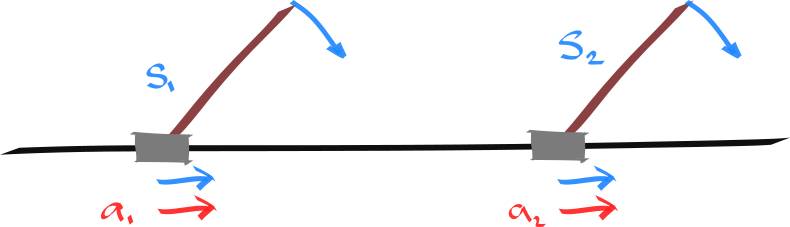
\includegraphics[width=1\textwidth,height=0.25\textheight]{../../pictures/drawings/cart-pole-translation.png}
\caption{???}
\end{figure}

(special case of regular actions)


\begin{align}
\Delta_{\tau}(s_1, a_1) = \Delta_{\tau}(s_1, a_2) = \Delta_{\tau}(s_2, a_1) = \Delta_{\tau}(s_2, a_2) \\
 \text{ if} \;\;\forall a\;\;\pi(a | s_1) = \pi(a| s_2) \\
Q_\pi(s_1, a_1) = Q_\pi(s_2, a_2)= Q_\pi(s_1, a_2) = Q_\pi(s_2, a_1) \\
\end{align}


\hypertarget{local-symmetry}{%
\subsubsection{Local symmetry}\label{local-symmetry}}

(\emph{this is approximately a symmetry})

\begin{figure}
\centering
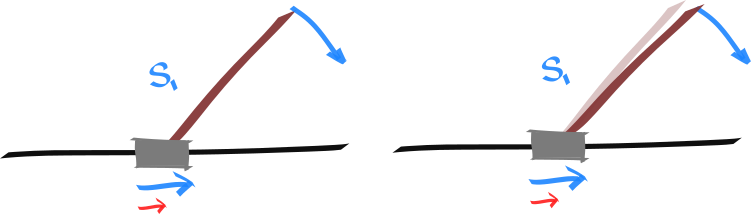
\includegraphics[width=1\textwidth,height=0.25\textheight]{../../pictures/drawings/cart-pole-approx.png}
\caption{???}
\end{figure}

\begin{align}
\Delta(s_1, a_1) = \Delta(s_1, a_2) = \Delta(s_2, a_1) = \Delta(s_2, a_2) \\
\forall a \text{ set}\;\;\pi(a | s_1) = \pi(a| s_2) \\
Q_\pi(s_1, a_1) \approx Q_\pi(s_2, a_2)  \\
\end{align}

\hypertarget{future-translational-symmetry}{%
\subsubsection{Future translational
symmetry}\label{future-translational-symmetry}}

\begin{figure}
\centering
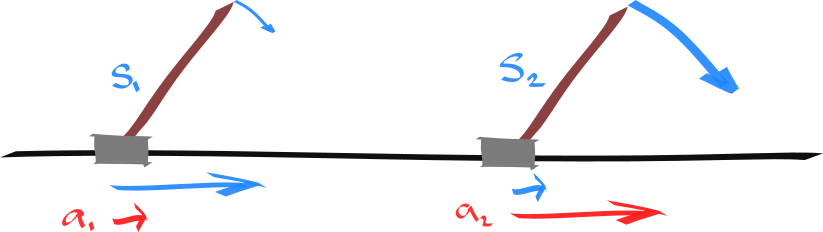
\includegraphics[width=1\textwidth,height=0.25\textheight]{../../pictures/drawings/cart-pole-state.png}
\caption{???}
\end{figure}

different states, different actions. but maps into translational
symmetry.

After this action. All future actions will have the same effect. In this
sense, these two state-actions are similar.

\begin{align}
\forall a: \mathop{\mathbb E}_{s' \sim p(\cdot| s_1, a_1)} [\Delta(s', a)] =  \mathop{\mathbb E}_{s' \sim p(\cdot| s_2, a_2)} [\Delta(s', a)] \\
\end{align}

\hypertarget{temporal-mirror-symmetry}{%
\paragraph{Temporal mirror symmetry}\label{temporal-mirror-symmetry}}

This is simply a result of the earlier mirror symmetry?!? (want to show
this!)

permutations of actions that yield similar outcomes.

\begin{figure}
\centering
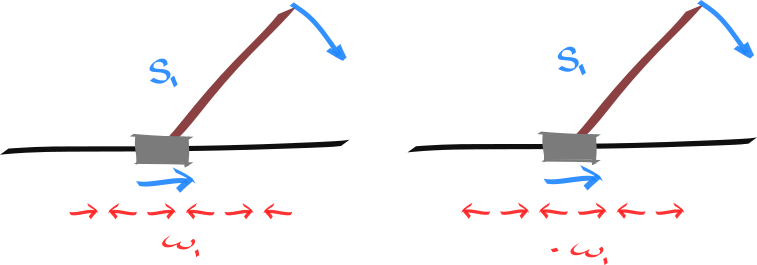
\includegraphics[width=1\textwidth,height=0.25\textheight]{../../pictures/drawings/cart-pole-temporal-mirror.png}
\caption{???}
\end{figure}

\begin{align}
p(s'|s, \omega) = \prod p(s|s, a)\omega(a|s) \\
p(\cdot|s_1, \omega_1) = p(\cdot|s_1, -\omega_1) \\
Q_{\pi}(s_1, \omega_1) = Q_{\pi}(s_1,-\omega_1) \\
\end{align}

\hypertarget{temporal-symmetry}{%
\paragraph{Temporal symmetry}\label{temporal-symmetry}}

\begin{figure}
\centering
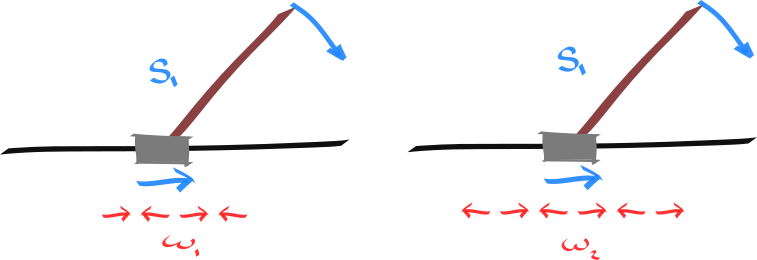
\includegraphics[width=1\textwidth,height=0.25\textheight]{../../pictures/drawings/cart-pole-temporal-approx.png}
\caption{???}
\end{figure}

\begin{align}
p(\cdot|s_1, \omega_1) = p(\cdot|s_1, \omega_2) \\
Q_{\pi}(s_1, \omega_1) = Q_{\pi}(s_1,\omega_2) \\
\end{align}

\hypertarget{pong}{%
\subsubsection{Pong}\label{pong}}

\hypertarget{mirror-symmetry-vertical}{%
\paragraph{Mirror symmetry (vertical)}\label{mirror-symmetry-vertical}}

\begin{figure}
\centering
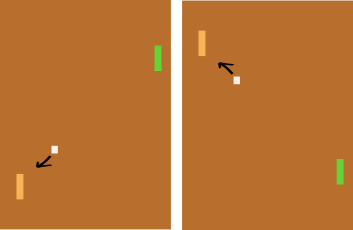
\includegraphics[width=1\textwidth,height=0.25\textheight]{../../pictures/drawings/pong-vert-flip.png}
\caption{???}
\end{figure}

(\emph{how can a change in state be evaluated? we need a
representation\ldots{}})

\begin{align}
\Delta_{T}(s, a) = (T \circ Q)(s,a) - Q(s,a)\\
\Delta_{T}(s_1, a_1) = \Delta_{T}(s_2, a_2) \\
\end{align}

\begin{align}
\forall a \text{ set}\;\;\pi(a | s_1) = \pi(-a| s_2) \\
Q_\pi(s_1, a_1) = Q_\pi(s_2, a_2) \\
Q_\pi(s_1, a_2) = Q_\pi(s_2, a_1) \\
\end{align}

\hypertarget{mirror-symmetry-horizontal}{%
\paragraph{Mirror symmetry
(horizontal)}\label{mirror-symmetry-horizontal}}

\begin{figure}
\centering
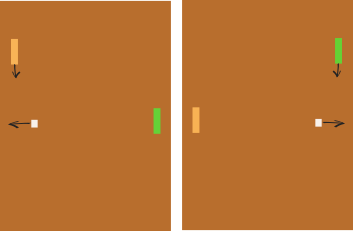
\includegraphics[width=1\textwidth,height=0.25\textheight]{../../pictures/drawings/pong-horz-flip.png}
\caption{???}
\end{figure}

Upon pretending to play as your opponent (flipping the image and
inverting the colors, via \(\rho: O \to O\), and ??? the actions)

\begin{align}
Q(s_1, a_1) = - V(\rho(s_2)) \\
\end{align}

(\emph{this really requires you to disentangle the model from your
opponent!?})

\begin{align}
\tau(s'|s, a_{p=0}) &= f_{p=0}(s''|s, a) \cdot f_{p=1}(s'|s'', \hat a) \cdot \pi_{p=1}(\hat a|s'') \\
Q_{p=0}(s, a) &= -Q_{p=1}(s, a)
\end{align}

\hypertarget{translational-symmetry-1}{%
\paragraph{Translational symmetry}\label{translational-symmetry-1}}

\begin{figure}
\centering
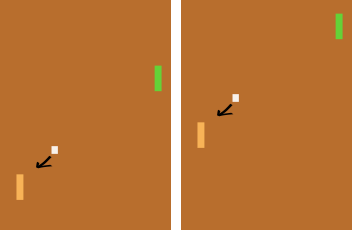
\includegraphics[width=1\textwidth,height=0.25\textheight]{../../pictures/drawings/pong-trans.png}
\caption{???}
\end{figure}

(\emph{although there are boundary cases which cannot be ignored. how
can they be dealt with!?})

\begin{align}
\forall a: Q_{\pi_1}(s_1, a) = Q_{\pi_2}(s_2, a) \\
\forall a, t: \pi_1(a|s^t_{s^0=s_1}) = \pi_2(a|s^t_{s^0=s_2})
\end{align}

If we take the same actions, in translated states, we get the same
outcome (up to the boundary conditions).

\hypertarget{temporal-symmetries}{%
\paragraph{Temporal symmetries}\label{temporal-symmetries}}

\begin{figure}
\centering
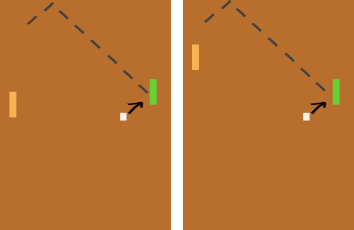
\includegraphics[width=1\textwidth,height=0.25\textheight]{../../pictures/drawings/pong-reach.png}
\caption{???}
\end{figure}

\begin{align}
\exists \pi_1, \pi_2 \;\;\text{s.t.} \;\; Q^{\pi_1}(s_1, a_1) = Q^{\pi_2}(s_2, a_2)
\end{align}

The same future state can be reached, and thus the same rewards can be
achieved.
